
\iffalse
\begin{forest}
  for tree={
    font=\ttfamily,
    grow'=0,
    child anchor=west,
    parent anchor=south,
    anchor=west,
    calign=first,
    inner ysep=0pt,
    edge path={
      \noexpand\path [draw, \forestoption{edge}]
      (!u.south west) +(20pt,0) |- node[fill,inner sep=5pt] {} (.child anchor)\forestoption{edge label};
    },
    before typesetting nodes={
      if n=1
        {insert before={[,phantom]}}
        {}
    },
    fit=band,
    before computing xy={l=40pt}, % Horizontal line length
  }
[
  [\myfolder{NXinstrument}
    [\myfolder{NXsource}]
    [\myfolder{NXdetector}
        [\myfile{counts[100]}]
        [\myfile{gas\_pressure[100]}]
        [\myfile{two\_theta[100]}]
        [\myfolder{NXoff\_geometry}
            [\myfile{vertices[100]}]
            [\myfile{faces[100]}]
        ]
    ]
    [\myfolder{NXmonochromator}]
  ]
  [\myfolder{NXdata}
    [\myfile{counts[100]}]
    [\myfile{two\_theta[100]}]
  ]
  [\myfolder{NXsample}]
]
\end{forest}
\fi

% \begin{figure}
% \caption{A typical nexus file layout with shape definition}
% 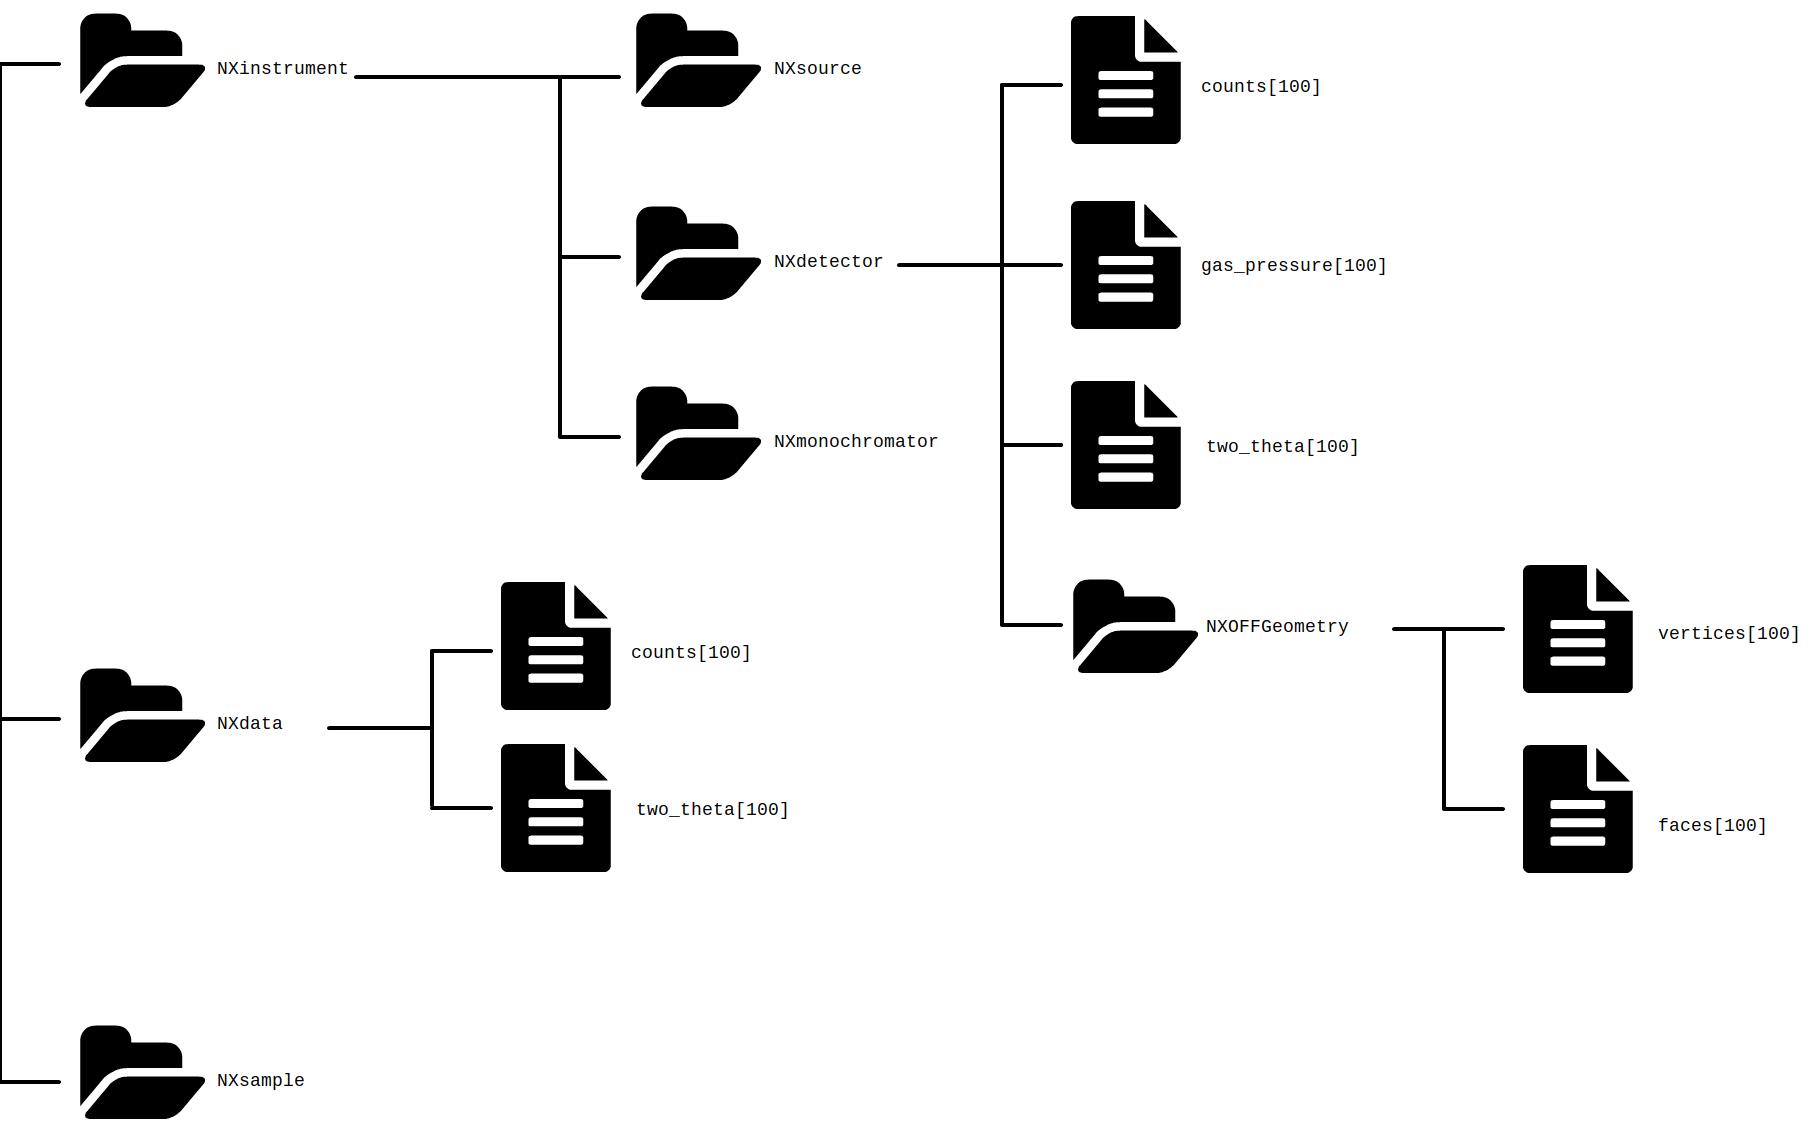
\includegraphics[width=\linewidth]{nexusdiagram.png}

% \end{figure}



% What's a shape definition?

A recent addition to the NeXus standard means components that are used in experiments can specify shape definition to describe their placement, size and geometry. Transformations (NXtransformations) can be applied to these components when their position changes during or before the experiment. 
